% ch12a Superconductivity in metals, part a (书页 189-204 / 分册p001-016)
% 第12章 Superconductivity in metals
\chapter{金属中的超导电性}

本章中，我们聚焦于超导电性现象及其背后的巴丁–库珀–施里弗（Bardeen–Cooper–Schrieffer，BCS）理论（文献 [BCS1957]）。当金属中有限比例的传导电子凝聚到一个由单一量子力学相位所表征的量子态上时，超导电性便出现了。这一量子力学相位的取值因超导体而异。把数量级达阿伏伽德罗常量之多的电子的相位锁定在一起，保证了超导态的刚性。例如，凝聚体中的电子不可能个别地运动；整个凝聚体作为一个单一的整体从样品的一端移动到另一端。同样，旨在破坏凝聚体的电子散射事件必须扰乱宏观数目电子的相位，才能摧毁超导态。因此，相位刚性既意味着超导凝聚体的集体运动，也意味着它的集体性毁灭。唯一另一个源于把宏观数目的粒子凝聚到相位锁定态的物理现象是玻色–爱因斯坦凝聚。然而，这两种效应之间有一个关键差别：构成超导凝聚体的粒子是库珀对（Cooper pair），它并不服从玻色统计。事实上，正是作用于组成库珀对的电子之上的泡利原理，阻止了把超导问题完全映射为一个简单的玻色凝聚问题。正如我们将看到的，正是泡利原理使 BCS 理论如此有效。这话是什么意思？在 BCS 理论中，假设电子形成库珀对，而且各对之间强烈地相互交叠。如此强的交叠本应意味着对与对之间存在强关联。事实上，正是对间的关联解释了超导体大多数可观测的性质，例如能隙和迈斯纳效应。然而在 BCS 理论中，库珀对之间并没有明确的动力学相互作用。唯一的相互作用——如果可以这样理解的话——来自泡利不相容原理，它禁止两个库珀对占据同一动量态。BCS 理论如此有效，这一事实深刻地揭示了金属中对–对关联的真实本质。它暗示金属中真实的对–对相互作用主要源于泡利不相容原理，而不是某种附加的动力学相互作用。正是主要因为这个原因，BCS 的简单配对假设才取得了如此深刻的成功。

\section{超导电性：唯象描述}

首先，我们摆明任何超导理论都必须解释的实验事实。

\begin{figure}[H]\centering
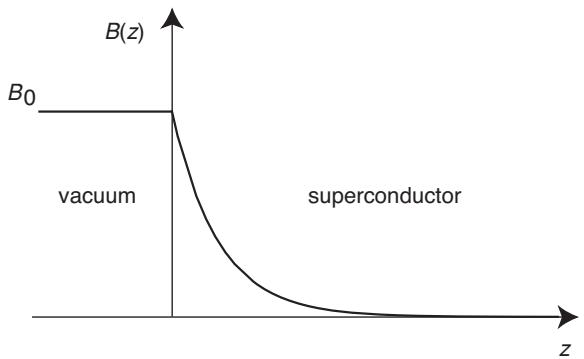
\includegraphics[width=0.5\textwidth]{figs/ch12/fig_12.1.jpg}
\caption*{图 12.1\quad 第I类超导体中磁场的衰减。}\label{fig:auto:12.1}
\end{figure}

\begin{figure}[H]\centering
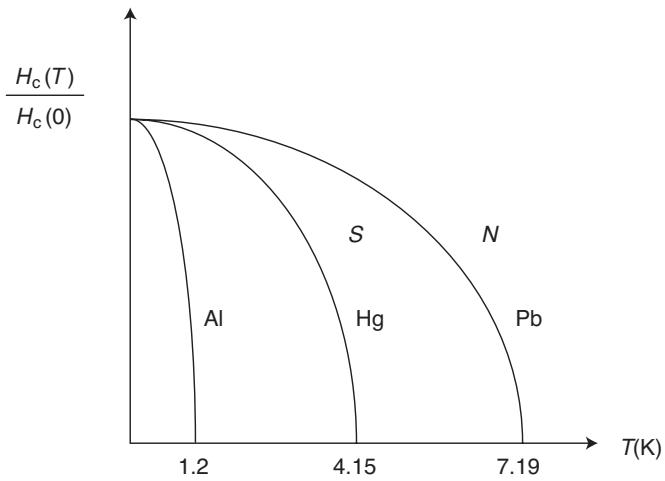
\includegraphics[width=0.55\textwidth]{figs/ch12/fig_12.2.jpg}
\caption*{图 12.2\quad 临界场随温度的依赖关系。横轴上标示的温度是一系列金属的超导转变温度。}\label{fig:auto:12.2}
\end{figure}

\textbf{(a) 零电阻}\quad 超导电性最典型的标志，是电阻在某个临界温度 $T_{\mathrm{c}}$ 以下消失。超导态是一个热力学上截然不同的物态。在 $T_{\mathrm{c}}$ 以下，电流的流动没有任何损耗。在高 $T_{\mathrm{c}}$ 材料被制备出来之前，铌（Nb）保持着最高的转变温度 $9.26\,\mathrm{K}$。

\textbf{(b) 迈斯纳效应}\quad 另一个特征是对磁场的排斥，即迈斯纳效应（Meissner effect）。迈斯纳效应完全的材料称为第I类超导体。因此，第I类超导体的内部是一个完全抗磁体。加在第I类超导体边界上的磁场，在材料内部随距离按指数衰减，如图12.1所示。穿透深度（penetration depth）$\lambda_{L}$ 定义为磁场衰减到 $1/e$ 倍所经过的距离。在 $T_{\mathrm{c}}$ 以下，破坏超导电性所需的场增大到某个临界值 $H_{\mathrm{c}}(T)$，如图12.2所示。由于超导体内部的磁场为零，
\begin{equation*}
B=0=H_{\mathrm{appl}}+4\pi M,\tag{12.1}
\end{equation*}
其中 $H_{\mathrm{appl}}$ 是外加场，$M$ 是磁化强度。解此方程，我们得到磁化强度为
\begin{equation*}
M=-\frac{1}{4\pi}H_{\mathrm{appl}}.\tag{12.2}
\end{equation*}
$M$ 的负值表明超导体内部是抗磁的。在低于 $T_{\mathrm{c}}$ 的任何温度下，磁化强度都应当是外加场的线性函数。具有这种形式磁化强度的材料称为第I类超导体。正常态用 N 表示，超导态用 S 表示。在 $H_{\mathrm{c}}$ 以上，$B\neq 0$，磁化强度不再服从式 (12.2)。

\begin{figure}[H]\centering
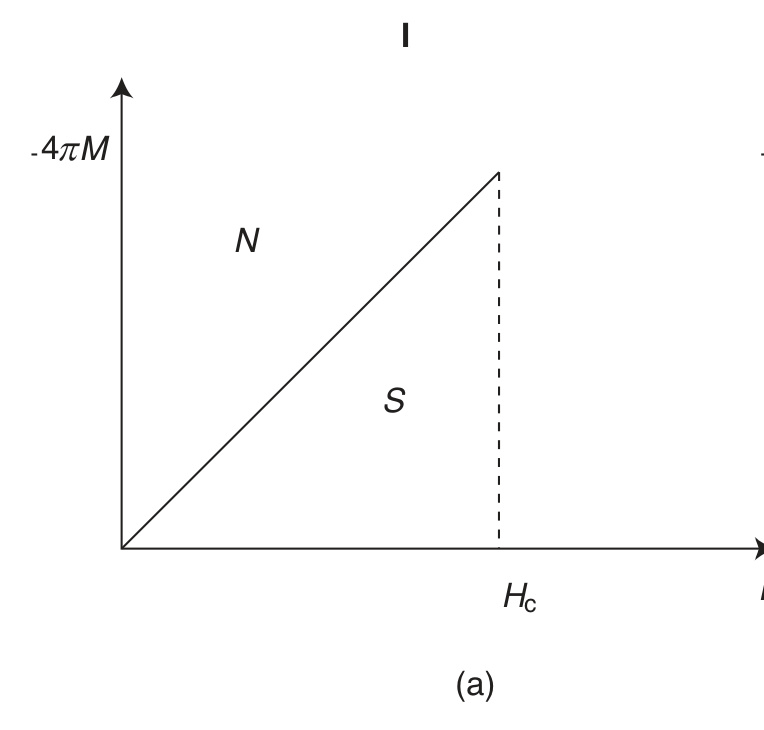
\includegraphics[width=0.48\textwidth]{figs/ch12/fig_12.3_a.jpg}\hfill
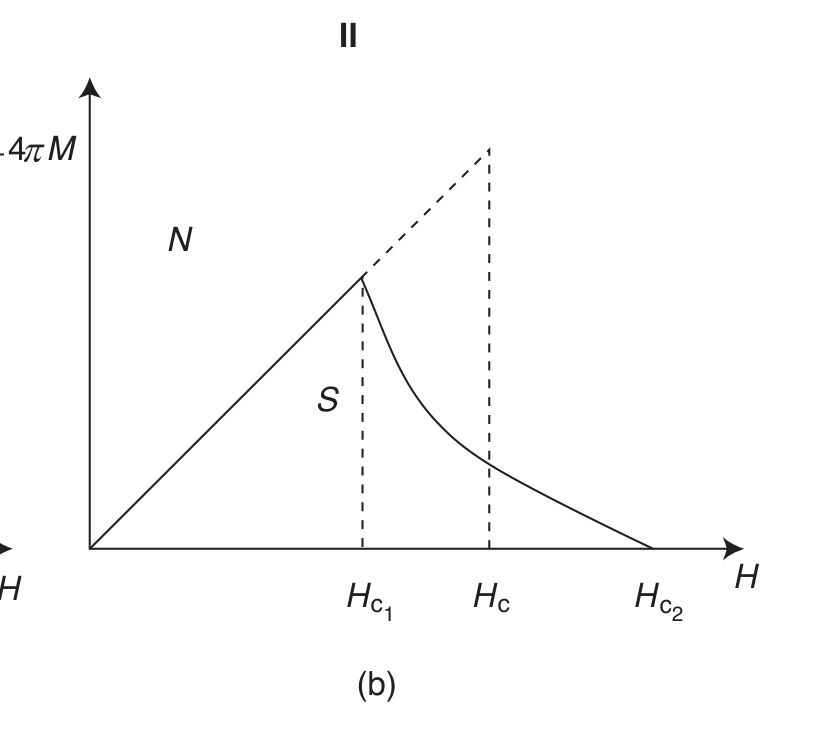
\includegraphics[width=0.48\textwidth]{figs/ch12/fig_12.3_b.jpg}
\caption*{图 12.3\quad (a) 第I类超导体的磁化强度对外加场的关系。(b) 第II类超导体的磁化强度对外加场的关系。在 $H_{\mathrm{c}_1}$ 与 $H_{\mathrm{c}_2}$ 之间，磁力线穿入超导体但并不破坏超导电性。磁力线形成一个涡旋晶格。}\label{fig:auto:12.3}
\end{figure}

在某些材料中，超导电性可以保持到上临界场 $H_{\mathrm{c}_2}$，但在下临界场 $H_{\mathrm{c}_1}$ 与 $H_{\mathrm{c}_2}$ 之间观察到的是不完全的迈斯纳效应。由此得到的磁化强度如图12.3(b)所示。表现出这种磁化强度的材料称为第II类超导体。在 $H_{\mathrm{c}_1}$ 与 $H_{\mathrm{c}_2}$ 之间，磁场穿入材料但超导电性并未被破坏。磁力线形成一个规则排列，称为阿布里科索夫（Abrikosov）涡旋晶格（文献 [A1957]）。所有高 $T_{\mathrm{c}}$ 铜氧化物超导体都是第II类的。

我们主要关心第I类材料。为理解超导体中的穿透深度，我们求助于伦敦（London）方程。首先，我们需要电场旋度的麦克斯韦方程：$-\partial\mathbf{B}/\partial t=c\nabla\times\mathbf{E}=c\rho\nabla\times\mathbf{J}$，其中 $\rho$ 是电阻率。在理想导体中 $\rho=0$，因而 $\partial\mathbf{B}/\partial t=0$。超导体中同样有 $\rho=0$。然而，实验事实是超导体内部 $B=0$。这一结果无法从麦克斯韦方程推出。正是迈斯纳效应把超导电性与仅显示理想导电性的材料区分开来。在超导体内部，磁通的排出由流动的电流所介导。伦敦于1935年提出，在超导体中处处有
\begin{equation*}
\mathbf{J}=-\mathrm{const.}\,\mathbf{A},\tag{12.3}
\end{equation*}
其中 $\mathbf{A}$ 是矢量势，$\mathbf{B}=\nabla\times\mathbf{A}$。由这个拟设（ansatz）出发，伦敦得以证明磁场在超导体内部按指数衰减。从量纲上看，该常数具有 $1/(L\cdot\text{时间})$ 的单位。我们把这个常数写成
\begin{equation*}
\mathrm{const.}=\frac{c}{4\pi\lambda_{L}^{2}},\tag{12.4}
\end{equation*}
其中 $c$ 是光速。对式 (12.3) 两边取旋度，我们得到
\begin{equation*}
\nabla\times\mathbf{J}=-\frac{c}{4\pi\lambda_{L}^{2}}\mathbf{B}.\tag{12.5}
\end{equation*}
由安培定律
\begin{equation*}
\nabla\times\mathbf{B}=\frac{4\pi}{c}\mathbf{j},\tag{12.6}
\end{equation*}
我们得到
\begin{equation*}
\nabla\times\left(\nabla\times\mathbf{B}\right)=\frac{4\pi}{c}\nabla\times\mathbf{J},\tag{12.7}
\end{equation*}
这意味着
\begin{equation*}
\nabla^{2}\mathbf{B}=\frac{1}{\lambda_{L}^{2}}\mathbf{B}.\tag{12.8}
\end{equation*}
此方程的解
\begin{equation*}
B(r)=B(0)\mathrm{e}^{-r/\lambda_{L}},\tag{12.9}
\end{equation*}
是在长度尺度 $\lambda_{L}$ 上按指数衰减的磁感应强度。磁场在超导体内的指数衰减就是迈斯纳效应。令 $v_{\mathrm{s}}$、$m^{*}$ 与 $e^{*}$ 分别是超导体中载流子的速度、质量和电荷。于是
\begin{equation*}
m^{*}\dot{\mathbf{v}}_{\mathrm{s}}=-e^{*}\mathbf{E}.\tag{12.10}
\end{equation*}
这些电子的电流定义为 $\mathbf{J}=-e^{*}\mathbf{v}_{\mathrm{s}}n_{\mathrm{s}}$，将它与式 (12.10) 联立，得到电流的时间演化方程
\begin{equation*}
\frac{\partial\mathbf{J}}{\partial t}=\frac{n_{\mathrm{s}}e^{*2}}{m^{*}}E\tag{12.11}
\end{equation*}
对两边取旋度，我们发现
\begin{align*}
0&=\frac{\partial}{\partial t}\left(\nabla\times\mathbf{J}\right)-\frac{n_{\mathrm{s}}e^{2}}{m^{*}}\nabla\times\mathbf{E}\\
&=\frac{\partial}{\partial t}\left(\nabla\times\mathbf{J}+\frac{n_{\mathrm{s}}e^{*2}}{m^{*}c}\mathbf{B}\right).\tag{12.12}
\end{align*}
将式 (12.12) 与式 (12.5) 比较，我们得到穿透深度为
\begin{equation*}
\lambda_{L}=\left(\frac{m^{*}c^{2}}{4\pi n_{\mathrm{s}}e^{*2}}\right)^{1/2}.\tag{12.13}
\end{equation*}
于是我们看到，随着超导密度的增大，$\lambda_{L}$ 减小。

我们可以借助金兹堡（Ginsburg）和朗道（Landau）的理论（文献 [GL1950]）来论证伦敦方法中的主要假设。这一唯象理论的关键之处在于：超导态与正常态之间自由能密度之差可以写成超导态序参量 $\psi(\mathbf{r})$ 的泛函。物理上，$|\psi(\mathbf{r})|^{2}$ 正比于超导态中的电荷密度 $n_{\mathrm{s}}$。因此，我们可以把 $\psi(\mathbf{r})$ 解释为超导态的波函数。在 BCS 理论中，$\psi(\mathbf{r})$ 扮演库珀对质心波函数的角色。在 $T_{\mathrm{c}}$ 附近，超流密度很小，故 $|\psi|^{2}\ll n_{\mathrm{e}}$。于是，金兹堡和朗道把超导态在 $T_{\mathrm{c}}$ 附近的自由能密度按 $|\psi|^{2}$ 的幂级数展开为
\begin{equation*}
F=F_{\mathrm{N}}+\int\mathrm{d}\mathbf{r}\left(\frac{\hbar^{2}}{2m^{*}}|\nabla\psi|^{2}+a(T)|\psi(\mathbf{r})|^{2}+b(T)|\psi(\mathbf{r})|^{4}\right),\tag{12.14}
\end{equation*}
其中保留了动能项 $|\nabla\psi|^{2}$，以显式地计入场 $\psi(\mathbf{r})$ 的空间变化。正常态的自由能是 $F_{\mathrm{N}}$。系数 $a(T)$ 与 $b(T)$ 是实的且依赖于温度，并且为使体系稳定，要求 $b(T)>0$。

为求系统的基态，我们对 $\psi^{*}(\mathbf{r})$ 极小化自由能密度：
\begin{equation*}
-\frac{\hbar^{2}}{2m^{*}}\nabla^{2}\psi(\mathbf{r})+a(T)\psi(\mathbf{r})+2b(T)|\psi(\mathbf{r})|^{2}\psi(\mathbf{r})=0.\tag{12.15}
\end{equation*}
由于自由能密度中含有恒为正的 $|\nabla\psi|^{2}$ 项，自由能的极小化要求 $\nabla\psi(\mathbf{r})=0$，或者说 $\psi$ 在空间中均匀。因此，鞍点方程的解要么是 $\psi=0$，要么是
\begin{equation*}
|\psi_{0}|^{2}=-\frac{a(T)}{2b(T)}=n_{\mathrm{s}},\tag{12.16}
\end{equation*}
这意味着 $a(T)<0$。倘若 $a(T)$ 大于零，则 $\psi=0$，系统将处于正常态。由于超导电性在 $T_{\mathrm{c}}$ 处消失，必须有 $a(T_{\mathrm{c}})=0$。把 $a(T)$ 在 $T_{\mathrm{c}}$ 附近作一阶泰勒展开，得到
\begin{equation*}
a(T)=a_{1}(T-T_{\mathrm{c}})\tag{12.17}
\end{equation*}
其中 $a_{1}>0$。

回忆起存在矢量势 $\mathbf{A}$ 时的电流密度为
\begin{equation*}
\mathbf{J}=\frac{e^{*}\hbar}{2\mathrm{i}m^{*}}\left(\psi^{*}\nabla\psi-\psi\nabla\psi^{*}\right)-\frac{e^{*2}}{m^{*}c}|\psi|^{2}\mathbf{A}.\tag{12.18}
\end{equation*}
若假定磁场足够小，以致 $\psi_{0}$ 的平衡值不变，则把 $\psi_{0}$ 代入式 (12.18) 便得到伦敦结果
\begin{equation*}
\mathbf{J}=-\frac{e^{*2}n_{\mathrm{s}}}{m^{*}c}\mathbf{A}.\tag{12.19}
\end{equation*}
利用式 (12.13)，我们发现这一结果与式 (12.4) 一致。于是，从这个简单的唯象方法出发，我们能够论证电流密度的伦敦拟设。的确，正如我们将看到的，BCS 超导理论的核心思想内容，正如在金兹堡–朗道理论中那样，是存在一个序参量，它描述一个具有确定相位的电荷 $2e$ 凝聚体。这样的凝聚体破坏 $U(1)$ 规范对称性，正如第1章所讨论的。事实上，迈斯纳效应的存在本身就意味着一个连续对称性的破缺。磁场无法穿入超导体这一事实立即告诉我们：在超导体中，光子是有质量的。因此，不能再假定电子是传播的自由度。实际上，在超导体中它们确实不是。电荷以 $2e$ 为单位量子化，这意味着 $U(1)$ 对称性发生了破缺。

\textbf{(c) 热容}\quad 在超导态中，熵连续但急剧地下降，标志着一种高度有序状态的形成。这描绘在图12.4(a)中。因此，熵对温度的导数在转变的超导一侧必然比正常一侧更陡。于是，热容在 $T_{\mathrm{c}}$ 处不连续，超导电性是一个二级相变。如图12.4(b)所示，在超导态中，热容 $c_{\mathrm{s}}$ 按 $c_{\mathrm{s}}\propto\exp(-\Delta/k_{\mathrm{B}}T)$ 衰减，其中 $\Delta$ 是一个能量尺度。这种形式的热容表明激发谱中存在能隙，且 $\epsilon_{p}>\mu$。让我们用一个简单的计算来验证这一点：
\begin{equation*}
c_{\mathrm{V}}=\frac{\partial}{\partial T}\int\frac{\epsilon_{p}\,\mathrm{d}\epsilon_{p}}{\left(\mathrm{e}^{\beta(\epsilon_{p}-\mu)}+1\right)}\overset{T\to 0}{\longrightarrow}\frac{\partial}{\partial T}\int\epsilon_{p}\,\mathrm{e}^{-\beta(\epsilon_{p}-\mu)}\,\mathrm{d}\epsilon_{p}.\tag{12.20}
\end{equation*}
若 $(\epsilon_{p}-\mu)\approx\Delta$，则 $c_{\mathrm{V}}\sim\exp(-\Delta(T=0)/k_{\mathrm{B}}T)$。因此，在超导态中，我们采用图12.5所示的能隙图像。

超导态中费米能级处能隙的形成导致系统基态能量的降低。能隙实际上是 $2\Delta$ 而非 $\Delta$。因此，$\epsilon_{p}-\mu$ 只占能隙的一半。实验上，能隙可以通过隧穿或超声衰减实验来测量。从热力学上看，能隙引起热容的不连续，即 $c_{\mathrm{s}}(T_{\mathrm{c}}^{-})-c_{\mathrm{N}}(T_{\mathrm{c}}^{+})\neq 0$。跨越超导转变时，自由能的两个一阶导数都为零，因此超导转变没有潜热。在 $T_{\mathrm{c}}$ 以上 $\Delta=0$，而在 $T=0$ 时 $\Delta$ 取其最大值。$\Delta(T)/\Delta(T=0)$ 的典型图像示于图12.6。弱耦合超导体的比值 $2\Delta(T=0)/k_{\mathrm{B}}T_{\mathrm{c}}$ 在 1 到 3 之间；强耦合对应于 $2\Delta(T=0)/k_{\mathrm{B}}T_{\mathrm{c}}>4$。在超导体中产生一个电子–空穴对所需的基本能量尺度是 $2\Delta$。

\begin{figure}[H]\centering
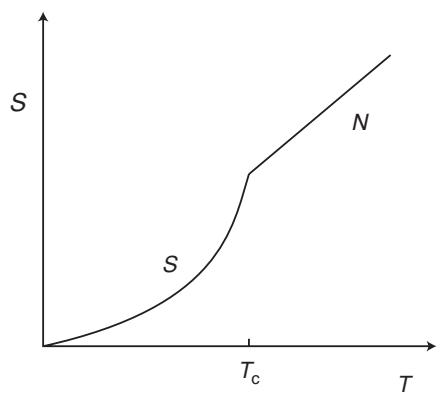
\includegraphics[width=0.48\textwidth]{figs/ch12/fig_12.4_a.jpg}\hfill
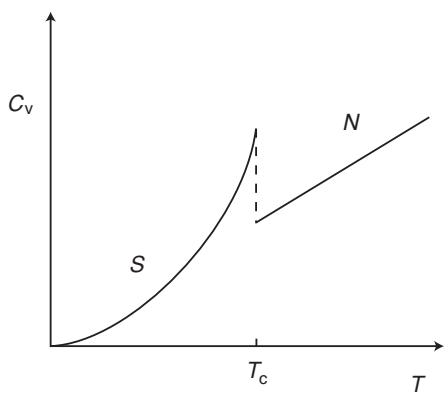
\includegraphics[width=0.48\textwidth]{figs/ch12/fig_12.4_b.jpg}
\caption*{图 12.4\quad (a) 熵在超导转变两侧的行为。(b) 正常态与超导态中热容的行为。}\label{fig:auto:12.4}
\end{figure}

\begin{figure}[H]\centering
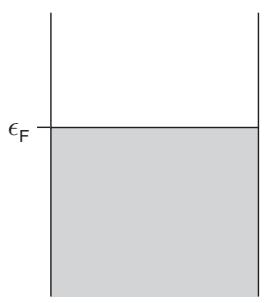
\includegraphics[width=0.42\textwidth]{figs/ch12/fig_12.5_a.jpg}\hfill
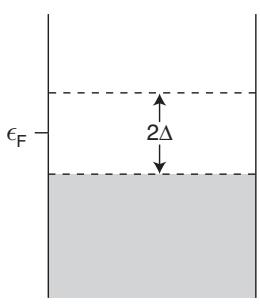
\includegraphics[width=0.42\textwidth]{figs/ch12/fig_12.5_b.jpg}
\caption*{图 12.5\quad (a) 正常态中被填满的能级。(b) 超导态中能隙的形成。完整的能隙是 $2\Delta$，而非 $\Delta$。}\label{fig:auto:12.5}
\end{figure}

\textbf{(d) 微波与红外性质}\quad 由于能隙的存在，能量小于 $2\Delta$ 的光子不会被吸收：所有这样的光子都被反射。当 $\omega<2\Delta(T=0)/\hbar$ 时发生完全反射。该条件成立时，光子看到的是一个完全无阻的表面。绝对零度下当 $\omega>2\Delta(T=0)/\hbar$ 时，电阻开始趋近正常态的值。我们在假定弱耦合描述对超导体适用的前提下估计这一能量：于是 $\Delta\sim 2k_{\mathrm{B}}T_{\mathrm{c}}$，而 $\omega\sim 4k_{\mathrm{B}}T_{\mathrm{c}}/\hbar$。对于 $T_{\mathrm{c}}=5\,\mathrm{K}$，$\omega\sim 10^{12}\,\mathrm{s}^{-1}$。这一频率位于红外波段。因此红外辐射可以穿入超导体并散射电子。

\begin{figure}[H]\centering
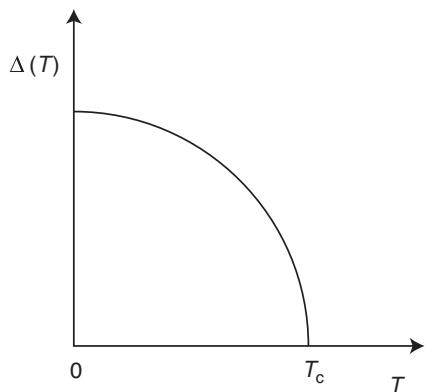
\includegraphics[width=0.5\textwidth]{figs/ch12/fig_12.6.jpg}
\caption*{图 12.6\quad 超导能隙 $\Delta$ 随 $T\to T_{\mathrm{c}}$ 的行为。}\label{fig:auto:12.6}
\end{figure}

\begin{figure}[H]\centering
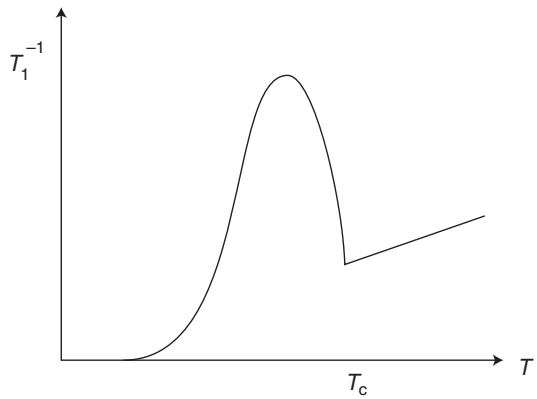
\includegraphics[width=0.5\textwidth]{figs/ch12/fig_12.7.jpg}
\caption*{图 12.7\quad $T_{\mathrm{c}}$ 处及 $T_{\mathrm{c}}$ 以下自旋–晶格弛豫时间的行为。$1/T_{1}$ 的增强是超导体中自旋协同行动的标志。}\label{fig:auto:12.7}
\end{figure}

\textbf{(e) 超声衰减}\quad 当 $\omega_{\mathbf{q}}<2\Delta/\hbar$ 时，入射声子束观察不到阻尼。与微波吸收的情形一样，$\omega_{\mathbf{q}}$ 必须超过产生一个电子–空穴对所需的能量。

\textbf{(f) 核自旋弛豫}\quad 考虑一组被强迫沿磁场排列的原子核。平衡磁化强度恢复的速率称为自旋–晶格弛豫速率 $1/T_{1}$。在超导体中，恰在 $T_{\mathrm{c}}$ 以下有 $\left(1/T_{1}\right)_{\mathrm{S}}>\left(1/T_{1}\right)_{\mathrm{N}}$。也就是说，超导态的形成带来弛豫速率的增强。Hebel 和 Slichter 最先在实验上观察到这一效应（文献 [HS1959]）。恰在 $T_{\mathrm{c}}$ 以下弛豫速率的峰称为 Hebel–Slichter 峰。

\textbf{(g) 同位素效应}\quad 实验上观察到，若以同位素方式改变离子的质量，$T_{\mathrm{c}}$ 会相应改变：
\begin{equation*}
T_{\mathrm{c}}\propto\frac{1}{\sqrt{M}}\propto\omega_{\mathrm{D}}.\tag{12.21}
\end{equation*}
这一观察表明，电子–声子耦合处于超导电性的核心（至少对传统超导电性是如此）。

\section{电子–声子有效相互作用}

$T_{\mathrm{c}}$ 的同位素依赖性证实了电子–声子耦合处于超导电性机制的中心。现在我们展示电子–声子耦合如何在两个电子之间产生吸引相互作用。我们分析的出发点是一个有序的电子能带，其中动能为 $\epsilon_{\mathbf{k}}$ 的电子与晶体的量子化振动模式相耦合。于是，我们的哈密顿量 $H=H_{o}+H_{\mathrm{e}\text{-}\mathrm{ph}}$ 由一个有序部分
\begin{equation*}
H_{o}=\sum_{\mathbf{q}}\hbar\omega_{\mathbf{q}}b_{\mathbf{q}}^{\dagger}b_{\mathbf{q}}+\sum_{\mathbf{k}}\epsilon_{\mathbf{k}}a_{\mathbf{k}}^{\dagger}a_{\mathbf{k}},\tag{12.22}
\end{equation*}
与电子–晶格相互作用
\begin{equation*}
H_{\mathrm{e}\text{-}\mathrm{ph}}=\sum_{\mathbf{k},\mathbf{q}}M_{\mathbf{q}}a_{\mathbf{k}+\mathbf{q}}^{\dagger}a_{\mathbf{k}}\bigl(b_{\mathbf{q}}+b_{-\mathbf{q}}^{\dagger}\bigr)\tag{12.23}
\end{equation*}
之和构成。

电子–声子耦合常数定义于第11.3节。我们将假定电子–声子相互作用是弱的，并对该相互作用做二阶微扰论。作为二阶微扰，我们预期电子–声子相互作用将给能量带来一个负的修正。虽然最终结果用二阶微扰论即可相当直接地建立起来（见习题12.3），但我们将采用相似变换（similarity transformation），因为该方法在电子–声子问题中有众多应用。我们的分析将仿照 Schrieffer–Wolff 变换。消去线性的电子–声子相互作用将产生一个二阶的相互作用，由此我们将能够推导出声子在何种条件下有效地束缚电子。

我们寻找一个变换 $S$，使得
\begin{equation*}
\left[H_{o},S\right]=-H_{\mathrm{e}\text{-}\mathrm{ph}}.\tag{12.24}
\end{equation*}
变换后的哈密顿量将为
\begin{align*}
\tilde{H}&=\mathrm{e}^{-S}H\mathrm{e}^{S}\\
&=H_{o}+\frac{1}{2}\left[H_{\mathrm{e}\text{-}\mathrm{ph}},S\right]+\cdots.\tag{12.25}
\end{align*}
我们设定 $S$ 具有如下形式
\begin{equation*}
S=\sum_{\mathbf{k},\mathbf{q}}\bigl(A_{\mathbf{k},\mathbf{q}}b_{-\mathbf{q}}^{\dagger}+B_{\mathbf{k},\mathbf{q}}b_{\mathbf{q}}\bigr)M_{\mathbf{q}}a_{\mathbf{k}+\mathbf{q}}^{\dagger}a_{\mathbf{k}},\tag{12.26}
\end{equation*}
其中 $A$ 与 $B$ 有待由式 (12.24) 的约束确定。为继续推进，我们需要对易关系
\begin{align*}
&\left[n_{\mathbf{k}},a_{\mathbf{k}_{1}}^{\dagger}a_{\mathbf{k}_{2}}\right]=a_{\mathbf{k}_{1}}^{\dagger}a_{\mathbf{k}_{2}}\left(\delta_{\mathbf{k}_{1}\mathbf{k}}-\delta_{\mathbf{k}_{2}\mathbf{k}}\right),\\
&\qquad\quad\ \left[b_{\mathbf{q}}^{\dagger},b_{\mathbf{q}}\right]=-1,\\
&\qquad\quad\ \left[b_{\mathbf{q}}^{\dagger}b_{\mathbf{q}},b_{\mathbf{q}'}\right]=-b_{\mathbf{q}}\delta_{\mathbf{q}\mathbf{q}'}.\tag{12.27}
\end{align*}
于是我们得到
\begin{align*}
\left[H_{o},S\right]&=\sum_{\mathbf{q}',\mathbf{k},\mathbf{q}}\hbar\omega_{\mathbf{q}'}\left[b_{\mathbf{q}}^{\dagger}b_{\mathbf{q}'},\bigl(A_{\mathbf{k},\mathbf{q}}b_{-\mathbf{q}}^{\dagger}+B_{\mathbf{k},\mathbf{q}}b_{\mathbf{q}}\bigr)a_{\mathbf{k}+\mathbf{q}}^{\dagger}a_{\mathbf{k}}\right]M_{\mathbf{q}}\\
&\quad+\sum_{\mathbf{k}',\mathbf{k},\mathbf{q}}\epsilon_{\mathbf{k}'}M_{\mathbf{q}}\left[a_{\mathbf{k}'}^{\dagger}a_{\mathbf{k}'},\bigl(A_{\mathbf{k},\mathbf{q}}b_{-\mathbf{q}}^{\dagger}+B_{\mathbf{k},\mathbf{q}}b_{\mathbf{q}}\bigr)a_{\mathbf{k}+\mathbf{q}}^{\dagger}a_{\mathbf{k}}\right]\\
&=\sum_{\mathbf{k},\mathbf{q}}M_{\mathbf{q}}b_{-\mathbf{q}}^{\dagger}a_{\mathbf{k}+\mathbf{q}}^{\dagger}a_{\mathbf{k}}\left(\hbar\omega_{-\mathbf{q}}+\epsilon_{\mathbf{k}+\mathbf{q}}-\epsilon_{\mathbf{k}}\right)A_{\mathbf{k},\mathbf{q}}\\
&\quad+\sum_{\mathbf{k},\mathbf{q}}M_{\mathbf{q}}b_{\mathbf{q}}a_{\mathbf{k}+\mathbf{q}}^{\dagger}a_{\mathbf{k}}\left(\epsilon_{\mathbf{k}+\mathbf{q}}-\epsilon_{\mathbf{k}}-\hbar\omega_{\mathbf{q}}\right)B_{\mathbf{k},\mathbf{q}}.\tag{12.28}
\end{align*}
该量必须等于 $-H_{\mathrm{e}\text{-}\mathrm{ph}}$。满足此约束的 $A_{\mathbf{k},\mathbf{q}}$ 与 $B_{\mathbf{k},\mathbf{q}}$ 系数为
\begin{equation*}
A_{\mathbf{k},\mathbf{q}}=-\bigl(\hbar\omega_{-\mathbf{q}}+\epsilon_{\mathbf{k}+\mathbf{q}}-\epsilon_{\mathbf{k}}\bigr)^{-1}\tag{12.29}
\end{equation*}
以及
\begin{equation*}
B_{\mathbf{k},\mathbf{q}}=-\bigl(\epsilon_{\mathbf{k}+\mathbf{q}}-\epsilon_{\mathbf{k}}-\hbar\omega_{\mathbf{q}}\bigr)^{-1}.\tag{12.30}
\end{equation*}
于是我们的幺正变换为
\begin{equation*}
S=\sum_{\mathbf{k},\mathbf{q}}\left[\frac{b_{-\mathbf{q}}^{\dagger}}{\left(\epsilon_{\mathbf{k}}-\epsilon_{\mathbf{k}+\mathbf{q}}-\hbar\omega_{-\mathbf{q}}\right)}+\frac{b_{\mathbf{q}}}{\left(\epsilon_{\mathbf{k}}-\epsilon_{\mathbf{k}+\mathbf{q}}+\hbar\omega_{\mathbf{q}}\right)}\right]M_{\mathbf{q}}a_{\mathbf{k}+\mathbf{q}}^{\dagger}a_{\mathbf{k}}.\tag{12.31}
\end{equation*}
注意能量分母的形式。$b_{-\mathbf{q}}^{\dagger}$ 的分母对应于发射能量为 $\hbar\omega_{-\mathbf{q}}$ 的声子时的能量差，而 $b_{\mathbf{q}}$ 的分母对应于吸收。我们定义 $\Delta_{\pm}(\mathbf{k},\mathbf{q})=\epsilon_{\mathbf{k}}-\epsilon_{\mathbf{k}+\mathbf{q}}\pm\hbar\omega_{\pm\mathbf{q}}$。有效哈密顿量由下式给出：
\begin{equation*}
\tilde{H}=H_{o}+\frac{1}{2}\sum_{\mathbf{k},\mathbf{q},\mathbf{k}',\mathbf{q}'}\left[M_{\mathbf{q}}M_{\mathbf{q}'}\Bigl(b_{-\mathbf{q}}^{\dagger}+b_{\mathbf{q}}\Bigr)a_{\mathbf{k}+\mathbf{q}}^{\dagger}a_{\mathbf{k}},\left(\frac{b_{-\mathbf{q}'}^{\dagger}}{\Delta_{-}(\mathbf{k}',\mathbf{q}')}+\frac{b_{\mathbf{q}'}}{\Delta_{+}(\mathbf{k}',\mathbf{q}')}\right)a_{\mathbf{k}'+\mathbf{q}'}^{\dagger}a_{\mathbf{k}'}\right].\tag{12.32}
\end{equation*}
我们需要计算形如下式的对易子
\begin{equation*}
\left[\bigl(b_{-\mathbf{q}}^{\dagger}+b_{\mathbf{q}}\bigr)a_{\mathbf{k}+\mathbf{q}}^{\dagger}a_{\mathbf{k}},b_{-\mathbf{q}'}^{\dagger}a_{\mathbf{k}'+\mathbf{q}'}^{\dagger}a_{\mathbf{k}'}\right].\tag{12.33}
\end{equation*}
具体地说，我们感兴趣的是由该对易子产生的两电子项。如果计算的是电子对易子部分，将只会得到一个单体势。这样的单体势在这里无关紧要，因为它们不影响两个电子之间的相互作用。涉及声子算符的对易子则产生一个有效的两体势，有趣的是，它在费米能附近一个窄的能量尺度内为负。为看清这一点，我们注意到式 (12.33) 中对易子的声子部分给出约束 $\delta_{\mathbf{q}+\mathbf{q}'}$。于是，我们的有效哈密顿量为
\begin{align*}
\tilde{H}&=H_{o}+\frac{1}{2}\sum_{\mathbf{k},\mathbf{k}',\mathbf{q}}M_{\mathbf{q}}M_{-\mathbf{q}}\left[\frac{a_{\mathbf{k}+\mathbf{q}}^{\dagger}a_{\mathbf{k}}a_{\mathbf{k}'-\mathbf{q}}^{\dagger}a_{\mathbf{k}'}}{\Delta_{-}(\mathbf{k}',-\mathbf{q})}-\frac{a_{\mathbf{k}+\mathbf{q}}^{\dagger}a_{\mathbf{k}}a_{\mathbf{k}'-\mathbf{q}}^{\dagger}a_{\mathbf{k}'}}{\Delta_{+}(\mathbf{k}',-\mathbf{q})}\right]\\
&=H_{o}+\sum_{\mathbf{k},\mathbf{k}',\mathbf{q}}\left|M_{\mathbf{q}}\right|^{2}a_{\mathbf{k}+\mathbf{q}}^{\dagger}a_{\mathbf{k}'-\mathbf{q}}^{\dagger}a_{\mathbf{k}'}a_{\mathbf{k}}\frac{\hbar\omega_{\mathbf{q}}}{\left(\Delta\epsilon_{\mathbf{k}',\mathbf{q}}\right)^{2}-\left(\hbar\omega_{\mathbf{q}}\right)^{2}}\tag{12.34}
\end{align*}
其中 $\Delta\epsilon_{\mathbf{k}',\mathbf{q}}=\epsilon_{\mathbf{k}'}-\epsilon_{\mathbf{k}'-\mathbf{q}}$。一般地，$\epsilon_{\mathbf{k}'}$ 与 $\epsilon_{\mathbf{k}'-\mathbf{q}}$ 远大于 $\hbar\omega_{\mathbf{q}}$。然而，若 $|\epsilon_{\mathbf{k}}-\epsilon_{\mathbf{k}-\mathbf{q}}|<\hbar\omega_{\mathbf{q}}$，则式 (12.34) 中的两电子势为负，电子感受到净吸引。注意，我们证明的是净吸引存在于 $k$ 空间而非实空间中。$k$ 空间中的吸引使两个电子得以束缚在一起，其总能量低于它们无相互作用时的情形。这一吸引是 BCS 超导电性中配对的基础。该相互作用的图形表示见图12.8，其中波浪线代表电子–声子相互作用
\begin{equation*}
V(\mathbf{k}',\mathbf{q})=\frac{\left|M_{\mathbf{q}}\right|^{2}\hbar\omega_{\mathbf{q}}}{\left(\epsilon_{\mathbf{k}'}-\epsilon_{\mathbf{k}'-\mathbf{q}}\right)^{2}-\left(\hbar\omega_{\mathbf{q}}\right)^{2}}.\tag{12.35}
\end{equation*}

\begin{figure}[H]\centering
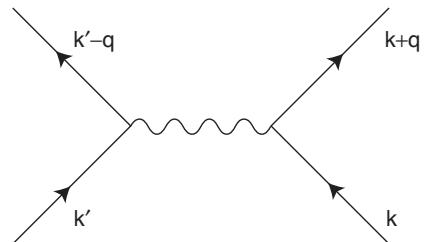
\includegraphics[width=0.55\textwidth]{figs/ch12/fig_12.8.jpg}
\caption*{图 12.8\quad 在费米面附近引起 BCS 配对的电子–声子相互作用。波浪线表示式 (12.35) 中的相互作用。}\label{fig:auto:12.8}
\end{figure}

\section{模型相互作用}

当然，在金属中我们还必须考虑电子–电子排斥。我们可以把这个势表示为
\begin{equation*}
V_{\mathrm{ee}}^{o}=\frac{V_{\mathrm{e}}(\mathbf{q})}{\varepsilon(\mathbf{q},\omega)},\tag{12.36}
\end{equation*}
其中 $\varepsilon(q,\omega)$ 是动态介电屏蔽函数。当然，电子–电子相互作用还有另一个来源，即由声子诱导的吸引。电子之间的完整相互作用具有如下形式
\begin{equation*}
V_{\mathrm{ee}}=\frac{V_{\mathrm{e}}(\mathbf{q})}{\varepsilon(\mathbf{q})}+\frac{\hbar\omega_{\mathbf{q}}\left|M_{\mathbf{q}}\right|^{2}}{\left(\Delta\epsilon_{\mathbf{k},\mathbf{q}}\right)^{2}-\left(\hbar\omega_{\mathbf{q}}\right)^{2}},\tag{12.37}
\end{equation*}
其中我们取了屏蔽函数的静态极限。现在 $\varepsilon(\mathbf{q})>0$，除非静态压缩率为负——如第9章所讨论的。这里我们排除这种情形，因为负压缩率出现在稀薄区间，那里需要对库仑相互作用作非微扰处理。通常，$V_{\mathrm{e}}(\mathbf{q})$ 远大于势的声子部分。然而，当 $\Delta\epsilon_{\mathbf{k},\mathbf{q}}\simeq\omega_{\mathbf{q}}$ 时，声子部分占主导，出现净吸引。于是我们看到，在不同的能量尺度上，声子部分或电子部分都可以占主导。相关的最大声子频率是 $\hbar\omega_{\mathrm{D}}$，即德拜能量。因此，当 $\Delta\epsilon_{\mathbf{k},\mathbf{q}}\le\hbar\omega_{\mathrm{D}}$ 时，产生的净吸引将压过电子排斥。当两个电子的能量都接近费米能量时，$\Delta\epsilon_{\mathbf{k},\mathbf{q}}\approx 0$，便得到吸引相互作用。这是 BCS 理论的一个本质特征。

在离开本节之前，考虑相互作用势 $V_{\mathrm{ee}}$ 的时间傅里叶变换是有益的。令 $\hbar\omega=\Delta\epsilon_{\mathbf{k},\mathbf{q}}$。$V_{\mathrm{ee}}$ 的傅里叶变换为
\begin{align*}
V_{\mathrm{ee}}(t)&=\int_{-\infty}^{\infty}\frac{\mathrm{d}\omega}{2\pi}\,\mathrm{e}^{-\mathrm{i}\omega t}\left[V_{\mathrm{ee}}^{o}+\frac{\hbar\omega_{\mathbf{q}}|M_{\mathbf{q}}|^{2}}{(\hbar\omega)^{2}-(\hbar\omega_{\mathbf{q}})^{2}}\right]\\
&=V_{\mathrm{ee}}^{o}\delta(t)+|M_{\mathbf{q}}|^{2}\frac{\hbar\omega_{\mathbf{q}}}{2\pi}\int_{-\infty}^{\infty}\frac{\mathrm{e}^{-\mathrm{i}\omega t}}{(\hbar\omega-\hbar\omega_{\mathbf{q}})(\hbar\omega+\hbar\omega_{\mathbf{q}})}\,\mathrm{d}\omega\\
&=V_{\mathrm{ee}}^{o}\delta(t)-|M_{\mathbf{q}}|^{2}\sin\omega_{\mathbf{q}}t.\tag{12.38}
\end{align*}

\begin{figure}[H]\centering
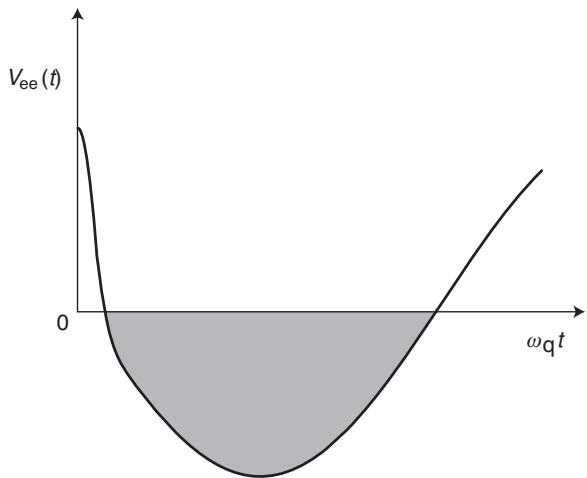
\includegraphics[width=0.6\textwidth]{figs/ch12/fig_12.9.jpg}
\caption*{图 12.9\quad 包含声子贡献的完整电子相互作用的傅里叶变换。电子排斥的 $\delta$ 函数贡献在 $t=0$ 附近被略微展宽。}\label{fig:auto:12.9}
\end{figure}

排斥部分只在 $t=0$ 起作用，而吸引部分是时间的振荡函数。总势示于图12.9。我们发现，电子势只在声子吸引占主导的那段时间间隔内是吸引的。这是关键的一点：时域中的 $V_{\mathrm{ee}}$ 并不总是吸引的。电子排斥与声子介导的吸引作用在不同的时间尺度上，因此电子的配对束缚是可能的。

让我们计算两体散射幅
\begin{equation*}
A_{\mathrm{s}}=\left\langle\mathbf{p}_{4\sigma_{1}}\mathbf{p}_{3\sigma_{2}}\right|V_{\mathrm{ee}}\left|\mathbf{p}_{1\sigma_{1}}\mathbf{p}_{2\sigma_{2}}\right\rangle,\tag{12.39}
\end{equation*}
其中
\begin{equation*}
V_{\mathrm{ee}}=\sum_{\mathbf{k},\mathbf{k}',\mathbf{q}}V(\mathbf{k},\mathbf{k}'-\mathbf{q})a_{\mathbf{k}+\mathbf{q}}^{\dagger}a_{\mathbf{k}'-\mathbf{q}}^{\dagger}a_{\mathbf{k}'}a_{\mathbf{k}}.\tag{12.40}
\end{equation*}
如第5章所讨论的，任何这种形式的两体幅都分解为直接与交换库仑积分之差。对一般的依赖动量的势，直接项与交换项将以动量和自旋的不同组合进入。例如，交换项将具有 $V(\mathbf{p}_{1},\mathbf{p}_{3})$ 的形式且 $\sigma_{1}=\sigma_{2}$，而直接项进入时对自旋没有限制，且依赖于 $V(\mathbf{p}_{1},\mathbf{p}_{4})$。让我们假定净吸引势是一个形如下式的常数
\begin{equation*}
V_{\mathrm{ee}}=\begin{cases}-V_{o}, & \left|\Delta\epsilon_{\mathbf{k}_{\mathrm{F}},\mathbf{q}}\right|<\hbar\omega_{\mathrm{D}},\\ 0, & \left|\Delta\epsilon_{\mathbf{k}_{\mathrm{F}},\mathbf{q}}\right|>\hbar\omega_{\mathrm{D}}.\end{cases}\tag{12.41}
\end{equation*}
由于势与动量无关，直接积分与交换积分相等，且当 $\sigma_{1}=\sigma_{2}$ 时散射幅为零。唯一非零的贡献来自 $\sigma_{1}\neq\sigma_{2}$。因此，对常数相互作用，只有当电子被锁定成单态时散射幅才非零。在这种情形下，声子在自旋相反的电子之间诱导出净吸引。相应的矩阵元形式为
\begin{equation*}
\left\langle\mathbf{p}_{4\uparrow}\mathbf{p}_{3\downarrow}\right|V_{\mathrm{ee}}\left|\mathbf{p}_{1\uparrow}\mathbf{p}_{2\downarrow}\right\rangle=-V_{0}\delta_{\mathbf{p}_{1}+\mathbf{p}_{2},\,\mathbf{p}_{3}+\mathbf{p}_{4}}\tag{12.42}
\end{equation*}
适用于费米面附近的散射。锁定成单态的两个粒子将在费米能级处产生能隙。

\section{库珀对}

现在考虑一个多少有些人为的问题：一个包含 $N$ 个无相互作用电子的满费米海，另有两个相互作用的电子处于海外。由于泡利不相容原理，费米海之外的电子其动量必须超过 $p_{\mathrm{F}}$。我们取相互作用势为上一节导出的常数单态对势，即式 (12.42)。于是自旋波函数对自旋是反对称的。相应的空间部分必须是对称的，以满足总体反对称性要求。我们这个两粒子子系统的本征值方程为
\begin{equation*}
\left[-\frac{\hbar^{2}}{2m}\bigl(\nabla_{1}^{2}+\nabla_{2}^{2}\bigr)+V(\mathbf{r}_{1}-\mathbf{r}_{2})-E\right]\Psi(\mathbf{r}_{1},\mathbf{r}_{2};\uparrow_{1},\downarrow_{2})=0.\tag{12.43}
\end{equation*}
一般地，两体波函数是一个复合态
\begin{equation*}
\Psi(\mathbf{r}_{1},\mathbf{r}_{2};\uparrow_{1},\downarrow_{2})=\psi(\mathbf{r}_{1},\mathbf{r}_{2})\chi_{S}(\uparrow_{1},\downarrow_{2}),\tag{12.44}
\end{equation*}
其中 $\chi_{S}(\uparrow_{1},\downarrow_{2})$ 表示单态自旋态，而 $\psi$ 包含空间依赖性。对两个粒子，我们可以用相对坐标 $\mathbf{r}=\mathbf{r}_{1}-\mathbf{r}_{2}$ 与质心 $\mathbf{R}=(\mathbf{r}_{1}+\mathbf{r}_{2})/2$ 把空间波函数表达为
\begin{equation*}
\psi(\mathbf{r}_{1},\mathbf{r}_{2})=\varphi(\mathbf{r})\,\mathrm{e}^{\mathrm{i}\mathbf{Q}\cdot\mathbf{R}/\hbar}.\tag{12.45}
\end{equation*}
同样，我们感兴趣的动量是质心动量 $\mathbf{Q}=\mathbf{p}_{1}+\mathbf{p}_{2}$ 与相对动量 $\mathbf{q}=(\mathbf{p}_{1}-\mathbf{p}_{2})/2$。我们把 $\varphi(\mathbf{r})$ 展开为傅里叶级数
\begin{equation*}
\varphi(\mathbf{r})=\sum_{\mathbf{k}}^{\prime}\frac{\mathrm{e}^{\mathrm{i}\mathbf{k}\cdot\mathbf{r}/\hbar}}{\sqrt{V}}\,\alpha_{\mathbf{k}},\tag{12.46}
\end{equation*}
其中撇号表示求和限于 $\mathbf{k}>\mathbf{k}_{\mathrm{F}}$，即所有能量超过 $\epsilon_{\mathrm{F}}$ 的态。由于 $\mathbf{k}\cdot\mathbf{r}=\mathbf{k}\cdot\mathbf{r}_{1}-\mathbf{k}\cdot\mathbf{r}_{2}$，我们看到对态具有动量 $(\mathbf{k},-\mathbf{k})$。注意，若 $\mathbf{k}_{1}+\mathbf{k}_{2}=0$，则质心运动从问题中消失。

我们首先关注 $\mathbf{Q}=0$ 的解。为此，我们定义相互作用势的傅里叶分量
\begin{equation*}
V_{\mathbf{k}\mathbf{k}'}=\int\frac{\mathrm{d}\mathbf{r}}{V}\,\mathrm{e}^{-\mathrm{i}(\mathbf{k}-\mathbf{k}')\cdot\mathbf{r}/\hbar}V(\mathbf{r}),\tag{12.47}
\end{equation*}
并引入质心薛定谔方程
\begin{equation*}
\left(-\frac{\hbar^{2}}{2\mu}\nabla^{2}+V(\mathbf{r})\right)\varphi(\mathbf{r})=E\varphi(\mathbf{r}),\tag{12.48}
\end{equation*}
其中 $\mu$ 是约化质量，$\mu=m/2$。代入 $\varphi(\mathbf{r})$ 的傅里叶表示，乘以 $\exp(-\mathrm{i}\mathbf{k}\cdot\mathbf{r}/\hbar)$ 并积分，我们得到
\begin{equation*}
\left(E-2\epsilon_{\mathbf{k}}\right)\alpha_{\mathbf{k}}=\sum_{\mathbf{k}'}V_{\mathbf{k}\mathbf{k}'}\alpha_{\mathbf{k}'}\tag{12.49}
\end{equation*}
作为我们的新本征值方程。这里 $\epsilon_{\mathbf{k}}=k^{2}/2m$。矩阵元 $V_{\mathbf{k}\mathbf{k}'}$ 等价于
\begin{equation*}
V_{\mathbf{k}\mathbf{k}'}=\left\langle\mathbf{k},-\mathbf{k}\right|V_{\mathrm{ee}}\left|\mathbf{k}',-\mathbf{k}'\right\rangle.\tag{12.50}
\end{equation*}
$V_{\mathbf{k}\mathbf{k}'}$ 中一个典型的散射过程示于图12.10。

\begin{figure}[H]\centering
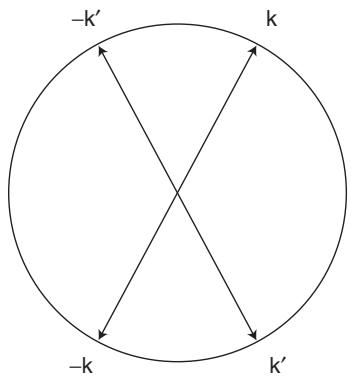
\includegraphics[width=0.5\textwidth]{figs/ch12/fig_12.10.jpg}
\caption*{图 12.10\quad 跨越费米面的一对电子态之间的散射。}\label{fig:auto:12.10}
\end{figure}

如果现在引入近似
\begin{equation*}
V_{\mathbf{k}\mathbf{k}'}=\begin{cases}-V_{0}, & k,k'>p_{\mathrm{F}},\\ 0, & \text{其余情形},\end{cases}\tag{12.51}
\end{equation*}
则本征值方程可以改写为
\begin{align*}
1&=-V_{0}\sum_{k>k_{\mathrm{F}}}\frac{1}{E-2\epsilon_{\mathbf{k}}}\\
&=-V_{0}\phi(E).\tag{12.52}
\end{align*}
只要 $\phi(E)=-1/V_{0}$，此方程即被满足。$\phi(E)$ 的极点位于 $E=2\epsilon_{\mathbf{k}}$，即该对的总能量，其下界为 $2\epsilon_{\mathrm{F}}$。在有限系统中，由于 $\mathbf{k}$ 是量子化的，$\epsilon_{\mathbf{k}}$ 取分立值。当 $E$ 从下方趋近 $2\epsilon_{\mathbf{k}}$ 时，$\phi(E)$ 趋于 $-\infty$；恰在 $2\epsilon_{\mathbf{k}}$ 上方，$\phi(E)$ 约为 $+\infty$。对所有 $E<2\epsilon_{\mathrm{F}}$，$\phi(E)$ 为负。因此，当 $\phi(E)$ 在 $E<2\epsilon_{\mathrm{F}}$ 处穿过 $-1/V_{0}$ 时，一个束缚态便形成了。$-1/V_{0}$ 与 $\phi(E)$ 的交点在图12.11中以图解方式给出。这种解的存在性就是库珀（Cooper）对问题（文献 [C1956]）。

\begin{figure}[H]\centering
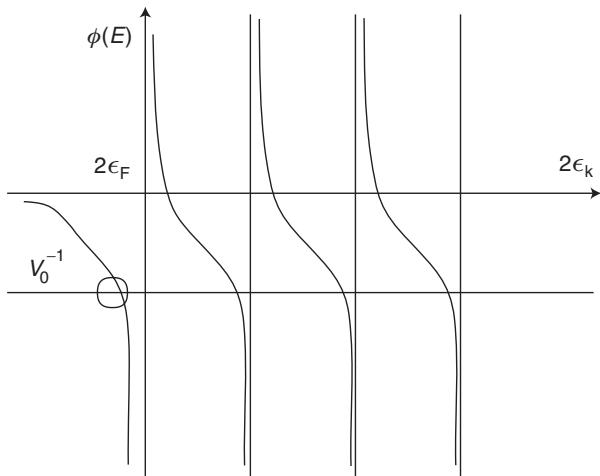
\includegraphics[width=0.62\textwidth]{figs/ch12/fig_12.11.jpg}
\caption*{图 12.11\quad 库珀对问题中 $\phi(E)$ 对 $\epsilon_{\mathbf{k}}$ 的图像。$\phi(E)$ 与直线 $-V_{0}^{-1}$ 的交点确定该对的束缚态解。}\label{fig:auto:12.11}
\end{figure}

为求出束缚态的精确能量，我们把式 (12.52) 中的求和换成积分，
\begin{equation*}
1=V_{0}\sum_{\epsilon(\mathbf{k})}^{\prime}\frac{1}{2\epsilon_{\mathbf{k}}-E}\ \to\ V_{0}\int_{\epsilon_{\mathrm{F}}}^{\epsilon_{\mathrm{F}}+\hbar\omega_{\mathrm{D}}}\frac{N(x)\,\mathrm{d}x}{2x-E}\tag{12.53}
\end{equation*}
其中引入了态密度 $N(x)$。若假定 $N(x)$ 在窄的积分区间内变化不大，则可取 $N(x)\approx N(\epsilon_{\mathrm{F}})$。在这些假设下，积分给出
\begin{equation*}
-\frac{2}{V_{0}N(\epsilon_{\mathrm{F}})}=\ln\left[\frac{\epsilon_{\mathrm{F}}-\frac{E}{2}}{\epsilon_{\mathrm{F}}-\frac{E}{2}+\hbar\omega_{\mathrm{D}}}\right],\tag{12.54}
\end{equation*}
由此可得
\begin{equation*}
\left(\epsilon_{\mathrm{F}}-\frac{E}{2}+\hbar\omega_{\mathrm{D}}\right)\exp\left(-\frac{2}{V_{0}N(\epsilon_{\mathrm{F}})}\right)=\epsilon_{\mathrm{F}}-\frac{E}{2}.\tag{12.55}
\end{equation*}
这个线性方程可以立即解出本征能量 $E$：
\begin{equation*}
E=2\epsilon_{\mathrm{F}}-\frac{2\hbar\omega_{\mathrm{D}}\exp\left(-2/V_{0}N(\epsilon_{\mathrm{F}})\right)}{1-\exp\left(-2/V_{0}N(\epsilon_{\mathrm{F}})\right)}.\tag{12.56}
\end{equation*}
在 $2\gg V_{0}N(\epsilon_{\mathrm{F}})$ 的极限下，分母中的指数函数可以展开。弱耦合极限下的对束缚能
\begin{equation*}
E\simeq 2\epsilon_{\mathrm{F}}-2\hbar\omega_{\mathrm{D}}\exp\left(-\frac{2}{V_{0}N(\epsilon_{\mathrm{F}})}\right)\tag{12.57}
\end{equation*}
随之得出。这两个表达式中的任何一个都表明：只要 $V_{0}$ 非零且为正，库珀对就以低于 $2\epsilon_{\mathrm{F}}$ 的能量束缚。这是一个深刻的结果。它意味着，只要存在式 (12.51) 形式的吸引相互作用，费米面正下方的两个电子可以通过被激发成动量为 $(\mathbf{k},-\mathbf{k})$、恰在费米面之上的库珀对而降低其能量。这就是所谓的库珀失稳（Cooper instability）。

进一步，我们可以估计对束缚能如何依赖于库珀对的质心。一开始我们猜想这个量可能按 $Q^{2}$ 标度。我们将证明并非如此。为推进讨论，我们把对束缚判据推广到 $Q\neq 0$ 的情形。对非零的 $Q$，该对的裸能量变为 $\epsilon_{\mathbf{q}+\mathbf{Q}/2}+\epsilon_{-\mathbf{q}+\mathbf{Q}/2}$。于是，对束缚条件变为
\begin{equation*}
1=-V_{0}\sum_{\mathbf{q}}\frac{1}{E-\epsilon_{\mathbf{q}+\mathbf{Q}/2}-\epsilon_{-\mathbf{q}+\mathbf{Q}/2}}.\tag{12.58}
\end{equation*}
对小的 $Q$，在略去 $O(Q^{2})$ 的项后，我们可以把式 (12.58) 改写为
\begin{equation*}
1=-V_{0}\int_{\epsilon_{\mathrm{F}}+v_{\mathrm{F}}Q/2}^{\epsilon_{\mathrm{F}}+v_{\mathrm{F}}Q/2+\hbar\omega_{\mathrm{D}}}\frac{N(\epsilon_{\mathbf{q}})\,\mathrm{d}\epsilon_{\mathbf{q}}}{E-2\epsilon_{\mathbf{q}}},\tag{12.59}
\end{equation*}
质心只不过移动了费米能量的零点。新的对束缚能
\begin{equation*}
E=2\epsilon_{\mathrm{F}}+Qv_{\mathrm{F}}-\frac{2\hbar\omega_{\mathrm{D}}}{\exp\left(2/V_{0}N(\epsilon_{\mathrm{F}})\right)-1},\tag{12.60}
\end{equation*}
是质心动量的线性函数。质心的平移会强烈地降低束缚能，最终可能拆散这个对。为说明这一点，我们令 $\epsilon_{\mathrm{F}}=0$，求出库珀对损失其大部分束缚能时的 $Q$ 值。我们必须求解
\begin{align*}
Qv_{\mathrm{F}}&=\frac{2\hbar\omega_{\mathrm{D}}}{\exp\left(2/V_{0}N(\epsilon_{\mathrm{F}})\right)-1}\\
&\approx k_{\mathrm{B}}T_{\mathrm{c}}.\tag{12.61}
\end{align*}
等价地，$Q/\hbar\sim k_{\mathrm{B}}T_{\mathrm{c}}/\hbar v_{\mathrm{F}}\sim 10^{4}\,\mathrm{cm}^{-1}$，大致是皮帕德（Pippard）相干长度 $\xi\sim 10^{-4}\,\mathrm{cm}$ 的倒数。这是库珀对的有效回转半径，与原子间距相比是一个巨大的距离。如此大的相干长度是声子配对机制的典型特征。
